
\section{Abstract}


\section{Introduction}

Drylands are at high risk of sudden desertification. This process of persistent vegetation loss is hardly understood but evidently a consequence of bistability. Under particular environmental conditions, two ecosystem states are likewise resilient to perturbations: One state with high vegetation cover of shrubs and grasses as well as a desert with no significant vegetation cover (Scheffer 2001). After crossing critical thresholds, or tipping-points, the system transites between the two stable states. 

For the dryland ecosystem, the major mechanism behind this bistability was found to be local facilitation of plant individuals. The presence of a plant provides its direct local environment with abilities of water retention, organic matter accumulation and protection against external stresses. When implemented in simple spatial models, This positive neighborhood effect provides true bistability on the landscape scale (K\'efi et al 2007a,b). 

This parent model was used before to investigate the consequences of increased plant mortality. This simple formulation of additional plant stress can be interpreted as the effects of increased grazing intensity by large herbivores (K\'efi et al 2007a). However, it is lacking some important features of grazing: the added plant mortality (1) applied globally, affecting all plants likewise, and (2) did not vary with vegetation density. The present study aims at increasing the realism of the model by applying two extensions that produce a more realistic gradient of grazing pressure on drylands. We provide a full factorial comparison of the consequences of these alternative models on vegetation structure and the ecosystems' bistability properties. The first extension adds the assumption of density dependent feeding. Grazers forage in the landscape and consume to fulfill their demands. At low density the grazing risk on individual plants will be high, while it will be shared among many plants when vegetation cover is high. For reasons of simplicity, we contrast the prior assumption of density independent individual risk with density independent global feeding. We expect this to consolidate the desert state by making it more resilient against recolonisation of single plants. The second extension implements an associative protection of plant individuals growing next to each other, a mechanism observed frequently among shrubs in dryland ecosystems. Here, the individual vulnerability against grazing is highest for plants growing isolated. The more direct neighbors a plant associates to, the lower is the effect of grazing. A plant in the patch center is not affected by grazing. We expect this mechanism to benefit the desert state, because at low densities only few plants are associated.



\section{Methods}
We used a cellular automaton to investigate the consequences of different grazing assumptions on the structural properties of the vegetation. This model was used before (Kefi et al 2007a, b) and can be resolved numerically in spatially explicit simulations but also analytically in differential equations. It defines landscape as a grid of cells, each can potentially take one of three discrete cell states: 'vegetated' cells are occupied by a plant individual (annotated as '+' in equations; black cells in figures); 'enriched' cells are suitable for seeds to germinate and colonise the cell, but do not contain adult plants right now  ('0' , grey cells); 'degraded' cells represent bare ground with lacking organic matter and bad water retention, and therefore can not be colonised by arriving seeds  ('$-$', white cells).
Transitions of cells states are only possible between vegetated and enriched (plant death / recolonisation) as well as enriched and degraded (degradation / regeneration). In biological terms, a degraded spot needs to be enriched first, before a plant can grow. Vice versa, when a plant dies, it leaves the spot in an enriched state, which might become degraded later. The rates for these transitions are defined in the following paragraphs. They might be constant values or functions of the global or local plant vegetation density (= $\rho_+$, global vegetation cover; $n_+$) .

\subsection{Facilitation model}
The original model by K\'efi et al mimics local facilitation of plants in drylands by defining the regeneration rate of degraded cells, $w_{ \left\{-,0 \right\} }$, as dependent on the density of vegetated cells in the nearest neighborhood, $\nu_+$ (assessing 'von Neumann'-neighborhood of range 1, i.e. the 4 nearest cells, $\nu_+ \in \left\{ 0, 0.25, 0.5, 0.75, 1 \right\}; $ K\'efi et al 2007b).
\begin{equation}
	w_{ \left\{-,0 \right\} } = r + \nu_{+} f
\end{equation}
% this is defining the rates of change of the population of cells in state '-'. 
%express rates rather as "probability of cell i,j to change into state x given that it is in state y".
The recolonisation of enriched cells takes into account that the majority of seeds arriving on a cell are from the plants in the direct neighborhood (local seed dispersal), while the probability of a successful plant establishment is limited by the competition on global resources.
\begin{equation}
	w_{ \left\{0,+ \right\} } = \left( \delta\rho_+ + \left( 1 - \delta \right)q_{+|0}\right) \left(b-c\rho_+ \right)
\end{equation}

%detailled description of parameters
The degradation of enriched cells is defined as a constant rate	
\begin{equation}
w_{ \left\{0,- \right\} } = d.
\label{eq:}
\end{equation}
Finally, in the original model, the intrinsic mortality of vegetated cells also is defined as constant $w_{ \left\{+,0 \right\} } = m$. Since it is defined as the probability of plant death per year, it also can be interpreted as inverse of the average lifespan of plants. However, the authors assume that this mortality might be increased by external stressors such as grazing. In the following paragraph, we explore different assumptions on how grazing affects the mortality of plant individuals.

\subsection{Grazer Models}
The \textbf{parent model} was used to explore consequences of increased plant mortality due to grazing. It simply adds grazing as a constant to individual mortality rate, affecting all plants homogenously.
\begin{equation}
	w_{ \left\{ +,0 \right\} }  = m_0 + g
\end{equation}
Therefore, $g$ . 

On the landscape scale, this means that vegetation loss due to grazing scales linearly with plant vegetation cover (Fig. 1a). However, while some stressors might change the intrinsic mortality of all plant individuals, independendly of the vegetation cover (e.g. fungal pests, drought), this is certainly not true for grazing.

Instead, in reality the impact of grazers varies strongly with plant vegetation cover. In the \textbf{livestock model}, we approximate the behaviourial responses of grazers to vegetation cover by the following assumption: The number of plants dying due to grazing should correspond to the biomass consumed by a number of grazers in the landscape, while being independent from vegetation cover  (Fig. 1b). Thus, individual risk is high, when few plants are present in the landscape and it is low for high vegetation cover. The correlation between vegetation density and individual risk is as follows. 
\begin{equation}
	w_{ \left\{ +,0 \right\} }  = m_0 + g_0 / \rho_+
\end{equation}
The two models therefore produce differing mortalities in cases departing from  $ \rho_+ = g_0 / g$. For densities $ \rho_+ < g_0 / g$, the livestock model produces higher mortality than the parent model. For $ \rho_+ > g_0 / g$, the opposite is the case. Since density is dynamic over time, with attractors depending on total individual ... 

To compare the two models, we define them to have equal mortality at intermediate vegetation cover, $\rho_+ = 0.5$. Therefore, in the parent model $g$ is set to be $g_0/0.5$. 

\subsection{Associative Protection}
Plants benefit from associative growth in an environment with physical stressors like grazing. Shrubs in particular shield each other from grazers when growing in direct neighborhood. Therefore plants growing isolated suffer more from grazing than plants growing within patches.
The models from the previous paragraph do not account for this locally differentiated impacts of grazing. To add \textbf{associative protection} to the model we need to define individual vulnerability, 
\begin{equation}
v = 1 - \nu_+ ,
\end{equation}
to decrease with the density of vegetated neighboring cells $\nu_+$. It is highest for isolated plants with no neighbors ($\nu_+ = 0$) and decreases linearly with the density of vegetated neighboring cells. A plant with four vegetated neighbors ($\nu_+ = 1$) is not vulnerable to grazing. 
To keep global grazing in accord to the parent model or the livestock model we normalize vulnerability against the average vulnerability of all vegetated cells,

\begin{equation}
\widehat{v} =  \frac{ \sum\limits_i{ 1 - {\nu_+i}}  } {n_+} ,
\label{eq:vul}
\end{equation}
yielding
\begin{equation}
	w_{ \left\{ +,0 \right\} }  = m_0 + g_0 / \rho_+ \frac{v}{\widehat{v}}.
\label{eq:}
\end{equation}

Therefore, we compare two spatial variants of grazing (spatially homogenous \textit{vs.} associative protection) for each grazer model (parent model with constant risk \textit{vs.} lifestock model with density dependent risk; see Table 1). 



\begin{table}[t!]
\label{tab:models}
\caption{the models' substitutions for grazing,  $g$, in the mortality term $w_{ \left\{ +,0 \right\} }  = m_0 + g$.  }
\centering
\begin{tabular}{ccc}

\toprule
 & parent model & lifestock model \\ \cmidrule(rl){2-2} \cmidrule(rl){3-3}
homogenous grazing &  $g_0/0.5$ & $g_0/\rho_+$\\
associative protection & $g_0/0.5 \frac{v}{\hat{v}}$  & $g_0/\rho_+ \frac{v}{\hat{v}}$ \\
	\bottomrule
\multicolumn{3}{p{9.5cm}}{\footnotesize $m_0$ : intrinsic mortality rate of vegetation, i.e. inverse of average lifespan, $g_0$: grazing intensity, $\rho_+$ : vegetation cover , $v$ : vulnerability, $\hat{v}$: mean vulnerability of all vegetated cells }
	\end{tabular}
\end{table}
%$n_+$ : number of vegetated cells on the lattice \par
%$\rho_+$ : global density of vegetated cells \par
%$\nu_n$ : density of neighbors in state n \par
%$g$ : grazing pressure



\subsection{Numerical simulations}

We apply these rules on a grid of 100 $\times$  100 cells of 0.25m$^2$ . The grid is defined to have periodic borders, connecting the east border to the west, the north to the south. Each timestep, which is defined as one year, the whole grid is updated synchronously multiple times, to increase stochasticity. At each update, the applicable transition probabilities for each single cell given in equations 1, 2, 3 and 4 are devided by the number of updates per year ( = 5) and tested against a uniform random number between 0 and 1. To initialize the grid with a standardized patch structure, each model simulation runs for 1.000 timesteps without any grazing using an initial environmental value $b_ini \in \left\{ 0.25, 3, 0.8, 0.9 \right\}$ before grazing is taking action (Note: I want to complete this to a highly resoluted gradient, to investigate the unstable equilibria). On those preconditioned grids, the four grazing models (Table ) run for 1.500 timesteps. An average vegetation cover, $\rho_+$, as well as the average cell mortality,$\hat{m}$ , is determined from the grids of the final 100 timesteps.


\subsection{Choice of parameters}

To investigate the bistability properties of the vegetation cover, we simulate a gradient in environmental quality b ranging from 0.2 to 1 with a step-width of 0.025. The models of this study inherit all parameters from the parent model in K\'efi et al. 2007a ($r = 0.01$, $f = 0.9$, $\delta = 0.1$, $c = 0.2$, $d = 0.1$), except the ones regarding mortality. We assume intrinsic mortality m0 for all models to be 0.5, re
ecting an average individual lifespan of 20 years, if no additional mortality due to grazing is taking effect. We investigate, how the stability properties and patch size distributions change over a grazing gradient.



\section{Results}

\newpage

\begin{figure}%
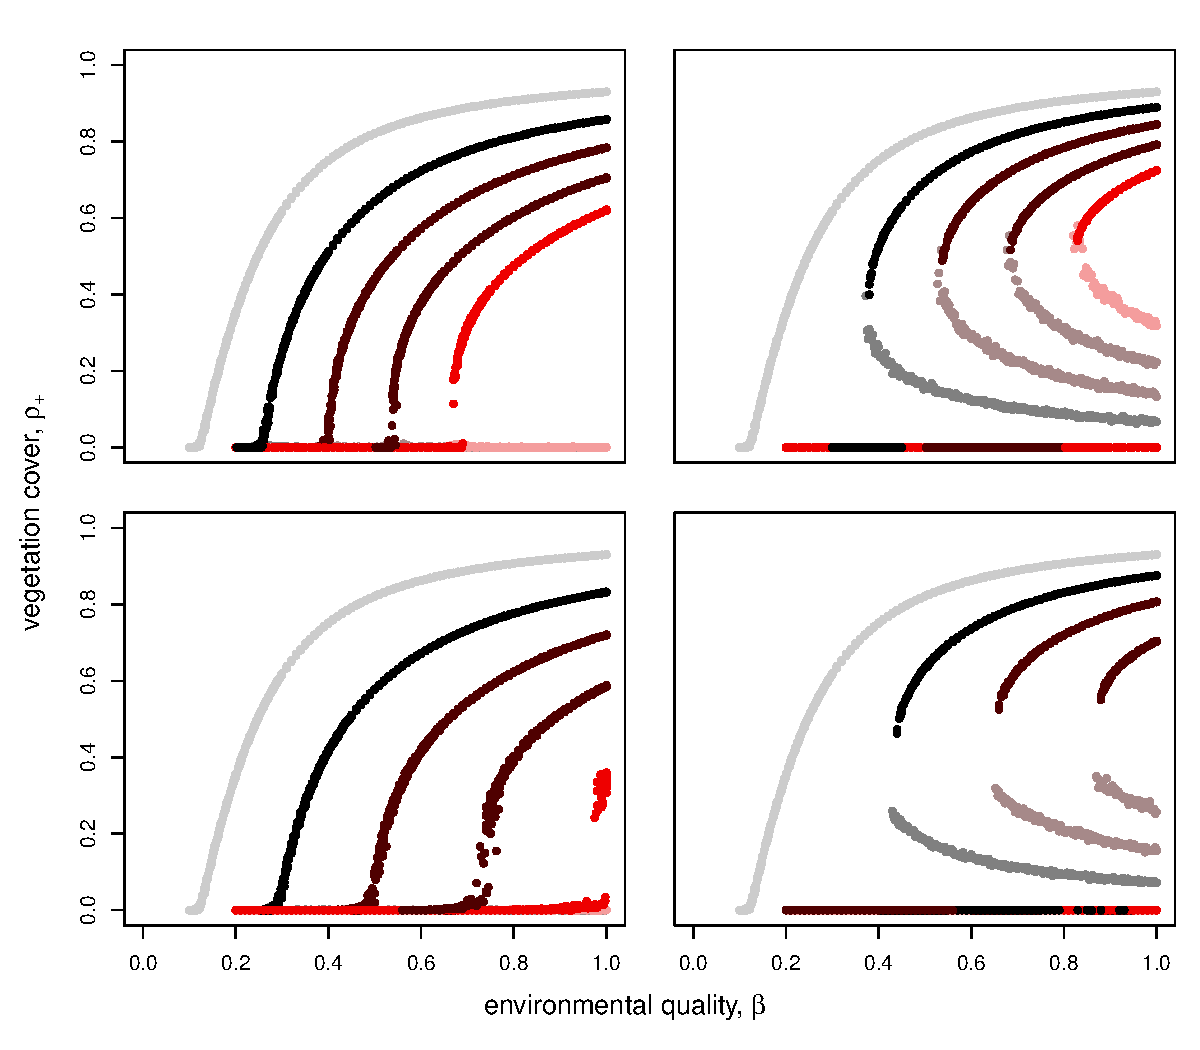
\includegraphics[width=\columnwidth]{figures/stability.pdf}%
\caption{Stable states of the vegetation cover, $\rho_+$, over gradient of environmental quality, $b$, under different grazing models. a) parent model with static, global grazing mortality, $g_0/0.5$. b) livestock model with density dependend, global grazing mortality, $g_0 / \rho_+$. c) associative protection model with differentiated grazing at patch border, $g_0/0.5 \frac{v}{\hat{v}}$ . d) livestock \& associative protection model with density dependend, differentiated grazing at patch border,  $g_0/ \rho_+ \frac{v}{\hat{v}}$ . Gradient of grazing intensity from grey: $g_0 = 0$, black to red: $g_0 \in \left\{ 0.025, 0.05, 0.075, 0.1 \right\}$.}%
\label{}%
\end{figure}



\section{Discussion}

Caveats
Functional response of large herbivores; Individual based, informed foraging


\section{Conclusion}
Undifferentiated model underestimates consequences of grazing with regard to the stability properties of the landscape. 
A linear increase in grazing causes shifts much  
